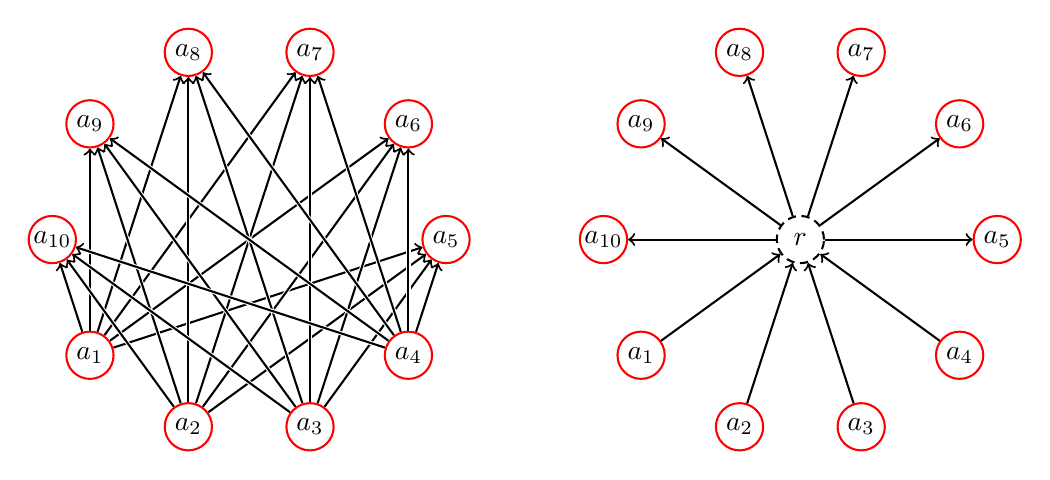
\begin{tikzpicture}[line width = 0.75pt,
                    basic/.style    = {circle, minimum size = 0.6cm, inner sep = 0pt, align = center},
                    attack/.style   = {draw = red,   basic},
                    resource/.style = {draw, densely dashed, basic},
                    function/.style = {draw = blue,  basic},
                    incident/.style = {draw = green, basic},
                    asset/.style    = {draw = black, basic}
                    ]
    \linespread{1}
    \uncover<2->{
    \foreach \i in {1, 2, ..., 10}
        \path (0,0) ++ (180 + 36*\i:2.5cm) node[attack] (aa\i) {$a_{\i}$};

    \foreach \i in {1, 2, 3, 4}{
        \foreach \j in {5, 6, ..., 10}{
            \draw[line width = 1.5pt, white] (aa\i) -- (aa\j);
            \draw[->] (aa\i) -- (aa\j);
        }
    }
    }
    
    \uncover<3>{
    \node[resource] (r) at (7, 0) {$r$};
    \foreach \i in {1, 2, ..., 10}
        \path (r) ++ (180 + 36*\i:2.5cm) node[attack] (a\i) {$a_{\i}$};

    \foreach \i in {1, 2, 3, 4}{
        \draw[->] (a\i) -- (r);
    }

    \foreach \i in {5, 6, ..., 10}{
        \draw[->] (r) -- (a\i);
    }
    }


    
\end{tikzpicture} 